%%%%%%%%%%%%%%%%%%%%%%%%%%%%%%%%%%%%%%%%%
% Beamer Presentation — SBPO 2026
% NS-BRKGA para o MOTMDSP
%%%%%%%%%%%%%%%%%%%%%%%%%%%%%%%%%%%%%%%%%

%----------------------------------------------------------------------------------------
%	PACKAGES AND OTHER DOCUMENT CONFIGURATIONS
%----------------------------------------------------------------------------------------

\documentclass[
	11pt,
	aspectratio=169, % 16:9 widescreen
]{beamer}

\graphicspath{{Images/}{figs/}{./}} % look for images in these directories

\usepackage{booktabs}
\usepackage{palatino}
\usepackage[default]{opensans}
\usepackage{graphicx}

% TikZ for diagrams
\usepackage{tikz}
\usetikzlibrary{arrows, arrows.meta, backgrounds, calc, fit, positioning, shapes}

%----------------------------------------------------------------------------------------
%	THEME CONFIGURATION
%----------------------------------------------------------------------------------------

\usetheme{CambridgeUS}
\usecolortheme{beaver}
\usefonttheme{default}
\useinnertheme{circles}

% Remove navigation symbols
\setbeamertemplate{navigation symbols}{}

% Show only frame number
\setbeamertemplate{page number in head/foot}[framenumber]

%----------------------------------------------------------------------------------------
%	CUSTOM COLOURS (PuOr palette)
%----------------------------------------------------------------------------------------

\definecolor{mydarkorange1}{RGB}{230, 97, 1}
\definecolor{mylightorange1}{RGB}{253, 184, 99}
\definecolor{mylightblue1}{RGB}{178, 171, 210}
\definecolor{mydarkblue1}{RGB}{94, 60, 153}
\definecolor{myorange3}{RGB}{229, 118, 26}
\definecolor{myblue3}{RGB}{127, 114, 180}
\definecolor{mygray}{RGB}{200, 200, 200}
\definecolor{mygreen}{RGB}{76, 169, 12}
\definecolor{mypurple}{RGB}{202, 162, 221}

%----------------------------------------------------------------------------------------
%	CUSTOM COMMANDS
%----------------------------------------------------------------------------------------

\newcommand{\NIGDplus}{\mathit{NIGD^{+}}}
\newcommand{\HVR}{\mathit{HVR}}
\newcommand{\takeaway}[1]{%
  \vspace{0.3em}
  \begin{center}
  \colorbox{mylightorange1!40}{\parbox{0.88\textwidth}{\centering\small\textbf{#1}}}
  \end{center}
}

%----------------------------------------------------------------------------------------
%	PRESENTATION INFORMATION
%----------------------------------------------------------------------------------------

\title[\textsc{NS-BRKGA} for MOTMDSP]{%
\textsc{NS-BRKGA} para o Multi-Objective\\
Time- and Machine-Dependent\\Scheduling Problem}

\author[Luis H. P. Mendes et al.]{%
Luis H. P. Mendes \and
F\'{a}bio L. Usberti \and
M\'{a}rio C. San Felice \and
Carlos E. de Andrade}

\institute[UNICAMP / UFSCar / AT\&T]{%
Institute of Computing -- University of Campinas (UNICAMP)\\
Department of Computing -- Federal University of S\~{a}o Carlos (UFSCar)\\
AT\&T Labs Research\\
\smallskip
\texttt{luis.mendes@ic.unicamp.br}}

\date[SBPO 2026]{LVIII Simp\'{o}sio Brasileiro de Pesquisa Operacional --- SBPO 2026}

%========================================================================================
\begin{document}

%========================================================================================
% TITLE SLIDE
%========================================================================================

\begin{frame}
\titlepage
\end{frame}

%========================================================================================
\section{Motivação}

%----------------------------------------------------------------------------------------
\begin{frame}
\frametitle{Veículos conectados precisam de atualizações de firmware}

\begin{columns}[c,onlytextwidth]
\column{0.55\textwidth}

\textbf{Firmware-Over-The-Air (FOTA):} atualização remota de software em
\textbf{milhões de veículos conectados} via rede celular.

~\\

Desafios principais:

\begin{itemize}
\item Veículos disponíveis apenas em \textbf{certos períodos} e \textbf{setores celulares}.

~\\

\item Cada setor tem \textbf{capacidade variável} no tempo.

~\\

\item Limite global de \textbf{largura de banda} por período.

~\\

\item Escala: até \textbf{10.000 jobs} ou \textbf{10.000 máquinas}.
\end{itemize}

\column{0.42\textwidth}
% TikZ: simplified vehicle availability diagram
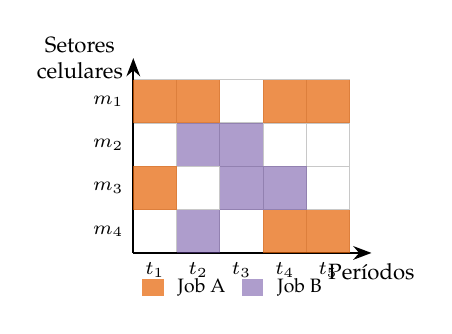
\begin{tikzpicture}[scale=0.55, font=\footnotesize]
  % Grid
  \draw[mygray] (0,0) grid[step=1] (5,4);
  % Axes
  \draw[-Stealth, thick] (0,0) -- (5.5,0) node[below] {Períodos};
  \draw[-Stealth, thick] (0,0) -- (0,4.5) node[left, align=center] {Setores\\celulares};
  % Vehicle availability blocks
  \fill[mydarkorange1, opacity=0.7] (0,3) rectangle (2,4);
  \fill[mydarkorange1, opacity=0.7] (3,3) rectangle (5,4);
  \fill[mydarkblue1, opacity=0.5] (1,2) rectangle (3,3);
  \fill[mydarkorange1, opacity=0.7] (0,1) rectangle (1,2);
  \fill[mydarkblue1, opacity=0.5] (2,1) rectangle (4,2);
  \fill[mydarkblue1, opacity=0.5] (1,0) rectangle (2,1);
  \fill[mydarkorange1, opacity=0.7] (3,0) rectangle (5,1);
  % Labels
  \node[left, font=\scriptsize] at (0,3.5) {$m_1$};
  \node[left, font=\scriptsize] at (0,2.5) {$m_2$};
  \node[left, font=\scriptsize] at (0,1.5) {$m_3$};
  \node[left, font=\scriptsize] at (0,0.5) {$m_4$};
  \foreach \t in {1,...,5} {
    \node[below, font=\scriptsize] at (\t-0.5, 0) {$t_{\t}$};
  }
  % Legend
  \fill[mydarkorange1, opacity=0.7] (0.2,-1.0) rectangle (0.7,-0.6);
  \node[right, font=\scriptsize] at (0.8,-0.8) {Job A};
  \fill[mydarkblue1, opacity=0.5] (2.5,-1.0) rectangle (3.0,-0.6);
  \node[right, font=\scriptsize] at (3.1,-0.8) {Job B};
\end{tikzpicture}
\end{columns}

\end{frame}

%----------------------------------------------------------------------------------------
\begin{frame}
\frametitle{Do FOTA ao TMDSP: um problema de escalonamento}

O cenário FOTA origina o \textbf{Time- and Machine-Dependent Scheduling Problem (TMDSP)}:

\smallskip

\begin{columns}[c,onlytextwidth]
\column{0.48\textwidth}
\begin{itemize}\setlength{\itemsep}{2pt}
\item \textbf{Jobs} = veículos a atualizar.
\item \textbf{Máquinas} = setores celulares.
\item \textbf{Períodos} = janelas de tempo discretas.
\item Capacidades \textbf{variam} por máquina e período.
\end{itemize}

\column{0.48\textwidth}
\begin{itemize}\setlength{\itemsep}{2pt}
\item Cada job atendido por \textbf{múltiplas máquinas} ao longo do tempo.
\item Restrições globais: banda, jobs ativos.
\item Objetivo original: minimizar $\sum_j C_j$.
\end{itemize}
\end{columns}

\smallskip

\takeaway{Mas minimizar apenas $\sum_j C_j$ não controla o makespan $C_{\max}$.\\
Alguns jobs podem terminar \textbf{muito mais tarde} que outros.}

\end{frame}

%----------------------------------------------------------------------------------------
\begin{frame}
\frametitle{MOTMDSP: dois objetivos conflitantes}

Propomos o \textbf{Multi-Objective TMDSP (MOTMDSP)}: minimizar \textbf{simultaneamente}:

\smallskip

\begin{columns}[c,onlytextwidth]
\column{0.48\textwidth}
\begin{block}{Makespan}
\[
\min \; C_{\max} = \max_{j \in J} C_j
\]
Último job a terminar.\\
\emph{Nenhum veículo espera demais.}
\end{block}

\column{0.48\textwidth}
\begin{block}{Tempo total de conclusão}
\[
\min \; \sum_{j \in J} C_j
\]
Soma de todos os tempos de conclusão.\\
\emph{Maximiza o throughput global.}
\end{block}
\end{columns}

\vspace{0.2em}

\begin{center}
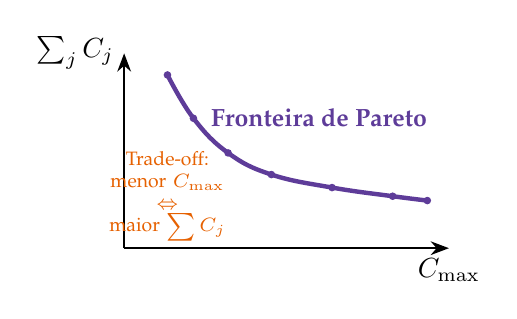
\begin{tikzpicture}[scale=0.55]
% Axes
\draw[-Stealth, thick] (0,0) -- (7.5,0) node[below] {$C_{\max}$};
\draw[-Stealth, thick] (0,0) -- (0,4.5) node[left] {$\sum_j C_j$};
% Pareto front curve
\draw[ultra thick, mydarkblue1, smooth, tension=0.7]
    plot coordinates {(1.0,4.0) (1.6,3.0) (2.4,2.2) (3.4,1.7) (4.8,1.4) (6.2,1.2) (7.0,1.1)};
% Points
\foreach \x/\y in {1.0/4.0, 1.6/3.0, 2.4/2.2, 3.4/1.7, 4.8/1.4, 6.2/1.2, 7.0/1.1} {
    \fill[mydarkblue1] (\x,\y) circle (2.5pt);
}
% Labels
\node[mydarkblue1, font=\small] at (4.5,3.0) {\textbf{Fronteira de Pareto}};
\node[mydarkorange1, font=\scriptsize, text width=2.5cm, align=center] at (1.0,1.2) {Trade-off:\\menor $C_{\max}$\\$\Leftrightarrow$\\maior $\sum C_j$};
\end{tikzpicture}
\end{center}

\end{frame}

%========================================================================================
\section{Método Proposto}

%----------------------------------------------------------------------------------------
\begin{frame}
\frametitle{NS-BRKGA = BRKGA + NSGA-II}

\textsc{NS-BRKGA} combina dois frameworks poderosos:

\smallskip

\begin{columns}[c,onlytextwidth]
\column{0.48\textwidth}
\textbf{De \textsc{BRKGA-MP-IPR}:}
\begin{itemize}\setlength{\itemsep}{2pt}
\item Cromossomo de \textbf{chaves aleatórias}
\item Crossover enviesado multi-parental
\item Path-relinking implícito
\item Shaking \& reset parcial
\end{itemize}

\column{0.48\textwidth}
\textbf{De \textsc{NSGA-II}:}
\begin{itemize}\setlength{\itemsep}{2pt}
\item \textbf{Non-dominated sorting}
\item \textbf{Crowding distance}
\item Seleção de elite baseada em Pareto
\end{itemize}
\end{columns}

\smallskip

\takeaway{O motor evolutivo é \textbf{independente do problema}.\\
Toda a lógica do MOTMDSP está no \textbf{decodificador}.}

\end{frame}

%----------------------------------------------------------------------------------------
\begin{frame}
\frametitle{Chaves aleatórias definem prioridades de escalonamento}

Um cromossomo é um vetor de valores reais:
\[
\mathbf{v} = (v_1, v_2, \ldots, v_{|J|}), \qquad v_j \in [0,\,1).
\]

\textbf{Decodificação:} ordenar jobs por valor \textbf{decrescente} da chave
$\Rightarrow$ define a \textbf{ordem de prioridade}.

~\\

\begin{center}
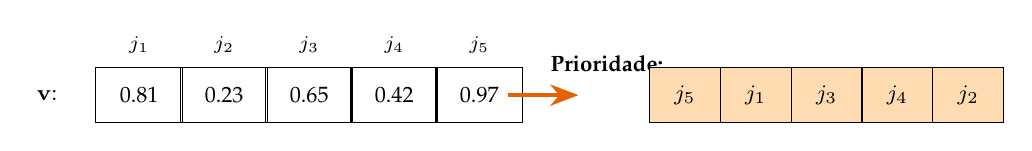
\begin{tikzpicture}[>=Stealth, scale=0.9]
% Chromosome
\node[font=\footnotesize] at (-1.3,0) {$\mathbf{v}$:};
\foreach \val [count=\i from 0] in {0.81, 0.23, 0.65, 0.42, 0.97} {
    \node[draw, minimum width=1.1cm, minimum height=0.7cm, font=\footnotesize]
        at (\i*1.2, 0) {\val};
    \node[font=\scriptsize, above] at (\i*1.2, 0.45) {$j_{\the\numexpr\i+1}$};
}

% Arrow
\draw[-Stealth, ultra thick, mydarkorange1] (5.2,0) -- (6.2,0);

% Priority
\node[font=\footnotesize] at (6.6,0.45) {\textbf{Prioridade:}};
\foreach \job [count=\i from 0] in {$j_5$, $j_1$, $j_3$, $j_4$, $j_2$} {
    \node[draw, fill=mylightorange1!50, minimum width=0.9cm, minimum height=0.7cm, font=\footnotesize]
        at (7.7+\i*1.0, 0) {\job};
}
\end{tikzpicture}
\end{center}

~\\

Pequenas perturbações nas chaves $\Rightarrow$ pequenas mudanças na ordem.\\
Permite \textbf{exploração suave} do espaço de permutações.

\end{frame}

%----------------------------------------------------------------------------------------
\begin{frame}
\frametitle{Decodificador: de prioridades a escalonamentos viáveis}

Dado um cromossomo $\mathbf{v}$, o decodificador constrói um \textbf{escalonamento viável left-shifted}:

\smallskip

\begin{enumerate}\setlength{\itemsep}{4pt}
\item \textbf{Ordenar} jobs por valor decrescente da chave.

\item Para cada job na ordem de prioridade:
    \begin{itemize}\setlength{\itemsep}{1pt}
    \item Alocar nos \textbf{primeiros intervalos máquina-período} viáveis.
    \item Respeitar capacidades $c_{mt}$, banda $r_{\max}$, limite $k_{\max}$.
    \item Continuar até a demanda $d_j$ ser totalmente atendida.
    \end{itemize}

\item Calcular $C_j$ para cada job, retornar $\mathbf{F} = (C_{\max},\; \sum_j C_j)$.
\end{enumerate}

\smallskip

\takeaway{O decodificador \textbf{sempre produz soluções viáveis}: sem reparo ou penalidade.}

\end{frame}

%----------------------------------------------------------------------------------------
\begin{frame}
\frametitle{Ciclo evolutivo do NS-BRKGA}

\begin{figure}
\centering
\scalebox{0.60}{
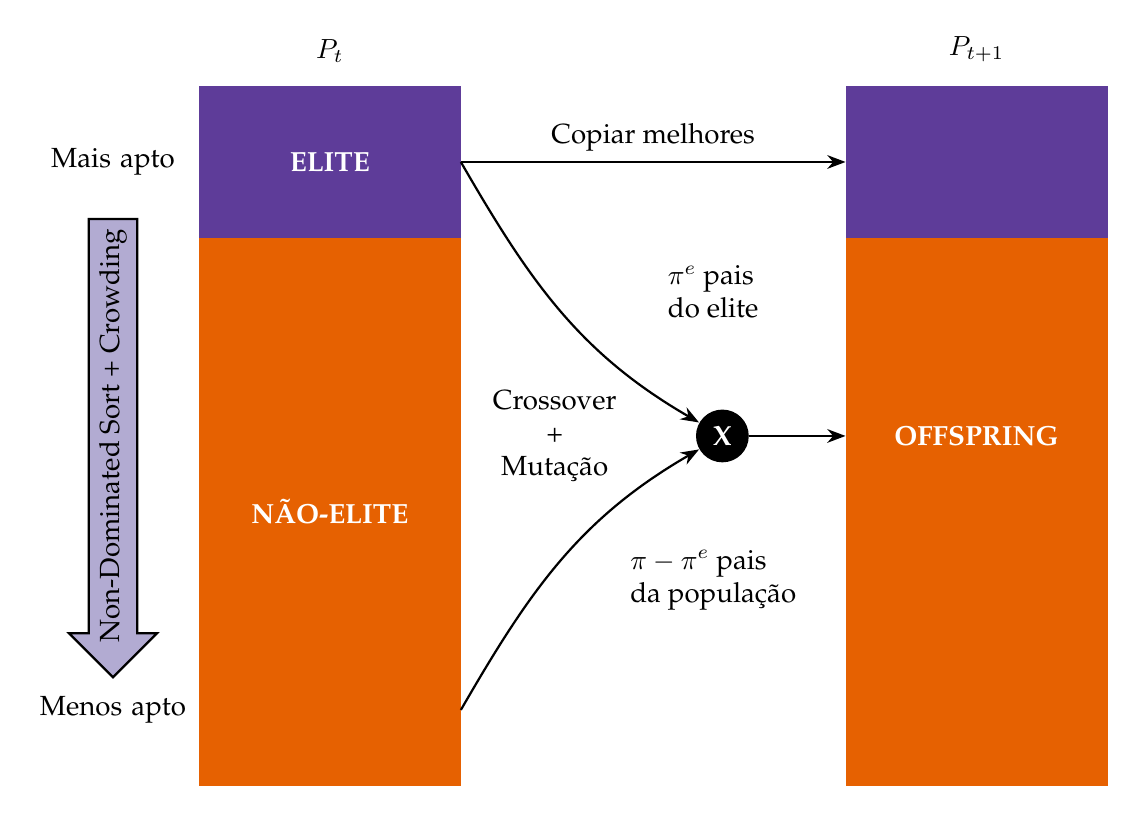
\begin{tikzpicture}
% --- Population Pt ---
\node [fill=mydarkblue1, text=white, text centered, outer sep=0, text width=88, minimum height=55, label={[yshift=5]north:$P_{t}$}] (elite) {\textbf{ELITE}};
\node at (elite.south) [anchor=north, fill=mydarkorange1, text=white, text width=88, text centered, minimum height=143, outer sep=0] (aux2) {};
\node at (elite.south) [anchor=north, fill=mydarkorange1, text=white, text width=88, text centered, minimum height=198, outer sep=0] (nonelite) {\textbf{NÃO-ELITE}};

% --- Population Pt+1 ---
\node at (elite.east) [anchor=west, fill=mydarkblue1, text=white, text centered, outer sep=0, text width=88, minimum height=55, xshift=139, label={[yshift=5]north:$P_{t + 1}$}] (top) {};
\node at (top.south) [anchor=north, fill=mydarkorange1, text=white, text centered, outer sep=0, text width=88, minimum height=198] (offspring) {};
\node at (top.south) [anchor=north, fill=mydarkorange1, text=white, text centered, outer sep=0, text width=88, minimum height=143] (middle) {\textbf{OFFSPRING}};
\node at (middle.south) [anchor=north, fill=mydarkorange1, text=black, text centered, outer sep=0, text width=88, minimum height=55] (bot) {};

\node at (bot.west) [anchor=east, fill=mydarkorange1, text=white, text centered, outer sep=0, text width=88, minimum height=55, xshift=-139] (aux) {};

% --- Sorting arrow ---
\node at (elite.west) [anchor=east, text width=55, text centered] (most) {Mais apto};
\node at (aux.west) [anchor=east, text width=55, text centered] (least) {Menos apto};
\node at($(most)!0.5!(least)$) [single arrow, draw=black, fill=white, thick, shape border rotate=180, rotate=90, fill=mylightblue1] (sort) {Non-Dominated Sort + Crowding};

% --- Crossover ---
\node at ($(aux2)!0.5!(middle)$) [circle, fill=black, text=white, text centered, xshift=25, label={[align=flush center, xshift=-25]west:Crossover \\ + \\ Mutação}] (crossover) {\textbf{X}};

% --- Arrows ---
\draw (elite) edge[-Stealth, thick, black] node[above] {Copiar melhores} (top);
\draw (elite.east) edge[-Stealth, thick, black, out=300, in=150] node[midway, align=flush left, xshift=55, yshift=07] {$\pi^{e}$ pais \\ do elite} (crossover);
\draw (aux.east) edge[-Stealth, thick, black, out=60, in=210] node[midway, align=flush left, xshift=55, yshift=-07] {$\pi - \pi^{e}$ pais \\ da população} (crossover);
\draw (crossover.east) edge[-Stealth, thick, black] (middle.west);
\end{tikzpicture}
}
\end{figure}

Adicionalmente: \textbf{múltiplas populações} com migração, \textbf{path-relinking} implícito, \textbf{shaking} em estagnação.

\end{frame}

%========================================================================================
\section{Experimentos Computacionais}

%----------------------------------------------------------------------------------------
\begin{frame}
\frametitle{Configuração experimental}

\begin{center}
\begin{tabular}{@{} l l @{}}
\toprule
\textbf{Parâmetro} & \textbf{Valor} \\
\midrule
Instâncias & \textbf{97} instâncias FOTA realistas \\
 & \quad 49 \texttt{common} + 48 \texttt{rare} \\
 & \quad até 10.000 jobs ou 10.000 máquinas \\
\addlinespace
Algoritmos & \textsc{NS-BRKGA} (proposto) \\
 & \textsc{NSGA-II}, \textsc{NSPSO}, \textsc{MOEA/D-DE}, \\
 & \textsc{MHACO}, \textsc{IHS} (PaGMO2) \\
\addlinespace
Execuções & 5 por algoritmo/instância \\
Tempo limite & 900\,s (15 min) por execução \\
Hardware & Intel Xeon E3-1230 V2, 32\,GB, 1 core \\
\addlinespace
Indicadores & $\NIGDplus$ (convergência, $\downarrow$) \\
 & $\HVR$ (convergência + diversidade, $\uparrow$) \\
\bottomrule
\end{tabular}
\end{center}

\vspace{0.3em}
{\small Fronteiras de referência: agregação de todas as soluções não-dominadas de \textbf{todos os algoritmos e execuções}.}

\end{frame}

%========================================================================================
\section{Resultados}

%----------------------------------------------------------------------------------------
\begin{frame}
\frametitle{NS-BRKGA atinge o melhor NIGD+ e HVR global}

\begin{figure}
\centering
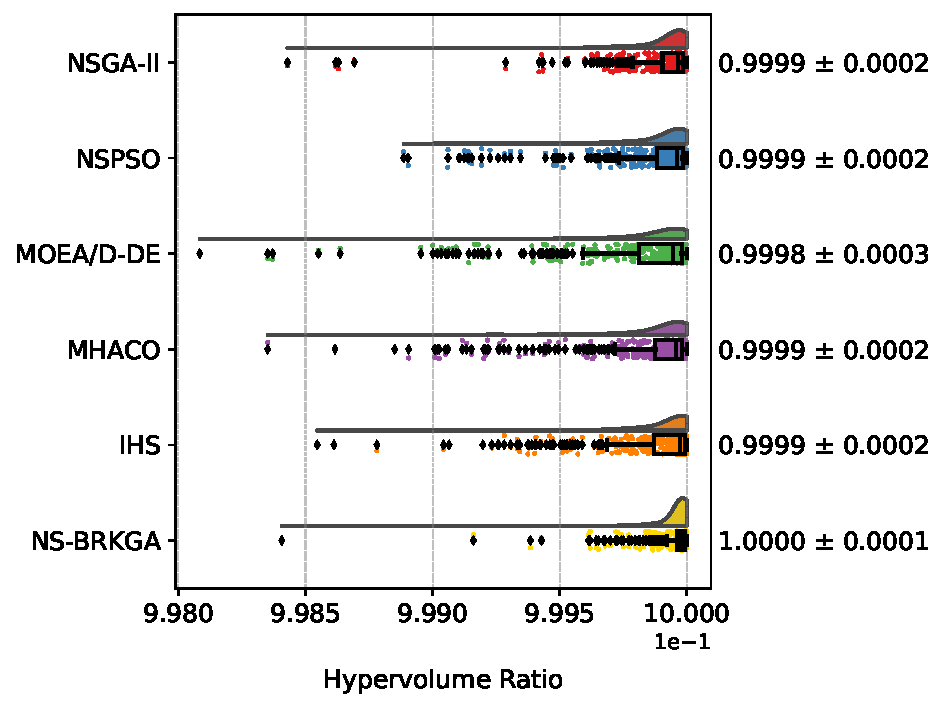
\includegraphics[width=0.42\textwidth]{figs/hypervolume.pdf}
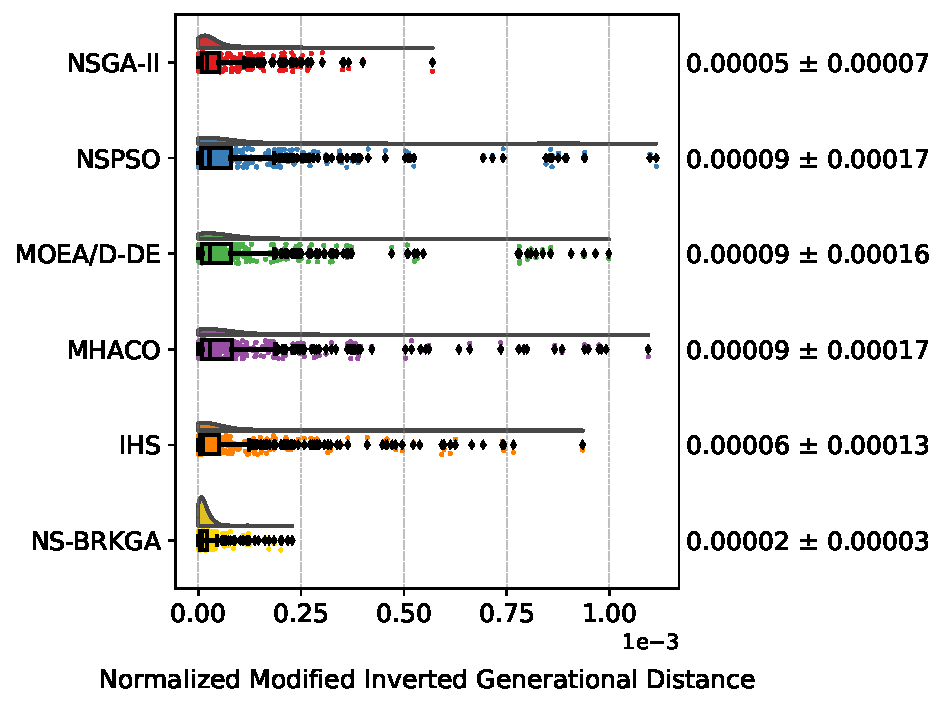
\includegraphics[width=0.42\textwidth]{figs/igd_plus.pdf}
\end{figure}

\begin{itemize}
\item $\HVR$: todos $\ge 0.999$ --- quase saturado, difícil diferenciar.
\item $\NIGDplus$ revela diferenças claras: \textsc{NS-BRKGA} atinge o \textbf{menor} $\NIGDplus$ final ($5{,}0 \times 10^{-5}$), seguido por IHS ($6{,}5 \times 10^{-5}$).
\end{itemize}

\takeaway{O $\NIGDplus$ diferencia melhor os algoritmos quando o $\HVR$ satura.}

\end{frame}

%----------------------------------------------------------------------------------------
\begin{frame}
\frametitle{Desempenho estável com o aumento da escala}

\begin{figure}
\centering
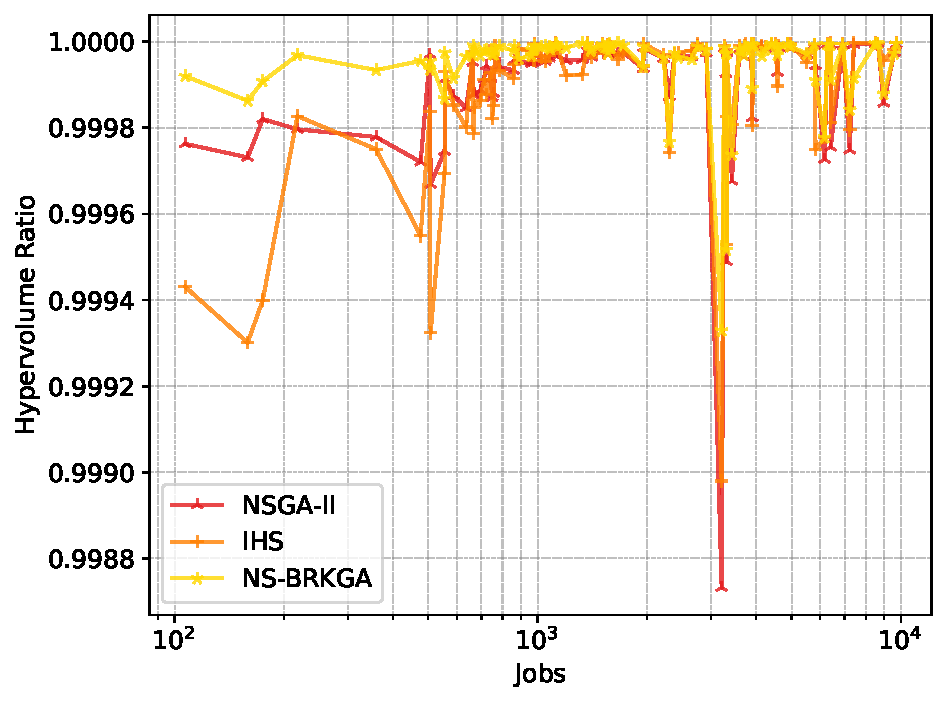
\includegraphics[width=0.42\textwidth]{figs/hypervolume_mean_per_jobs.pdf}
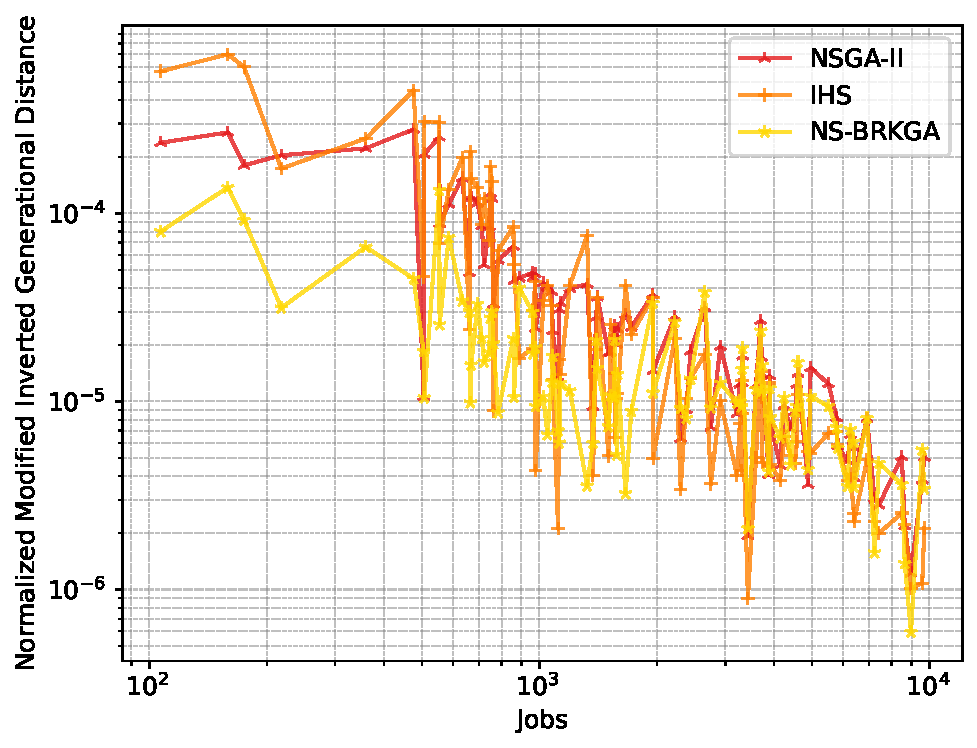
\includegraphics[width=0.42\textwidth]{figs/igd_plus_mean_per_jobs.pdf}
\end{figure}

\begin{itemize}
\item $\HVR$ permanece próximo de $1{,}0$ e $\NIGDplus$ baixo em todas as escalas.
\item \textbf{Sem degradação} ao aumentar o número de jobs.
\item \textsc{NS-BRKGA} consistentemente entre as melhores curvas.
\end{itemize}

\end{frame}

%----------------------------------------------------------------------------------------
\begin{frame}
\frametitle{Instâncias \texttt{rare}: onde NS-BRKGA mais se destaca}

\begin{columns}[c,onlytextwidth]
\column{0.48\textwidth}
\textbf{Instâncias \texttt{common}:}
\begin{itemize}\setlength{\itemsep}{1pt}
\item Todos os métodos: desempenho \textbf{similar}.
\item $\HVR \approx 1$, $\NIGDplus \sim 10^{-5}$.
\end{itemize}

\smallskip

\textbf{Instâncias \texttt{rare}:}
\begin{itemize}\setlength{\itemsep}{1pt}
\item Convergência \textbf{mais difícil}.
\item \textsc{NS-BRKGA}: $\NIGDplus = 2{,}5 \times 10^{-5}$ (\textbf{rank 1}).
\item Baselines: $8 \times 10^{-5}$ a $1{,}6 \times 10^{-4}$.
\end{itemize}

\column{0.48\textwidth}
\begin{figure}
\centering
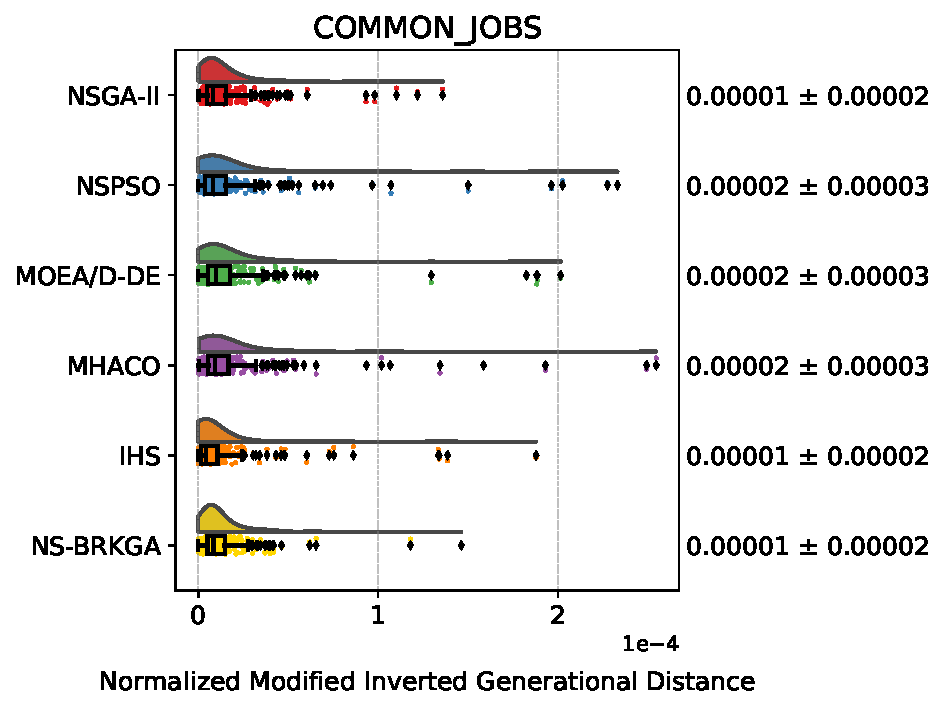
\includegraphics[width=0.88\textwidth]{figs/igd_plus_common_jobs.pdf}\\[0.2em]
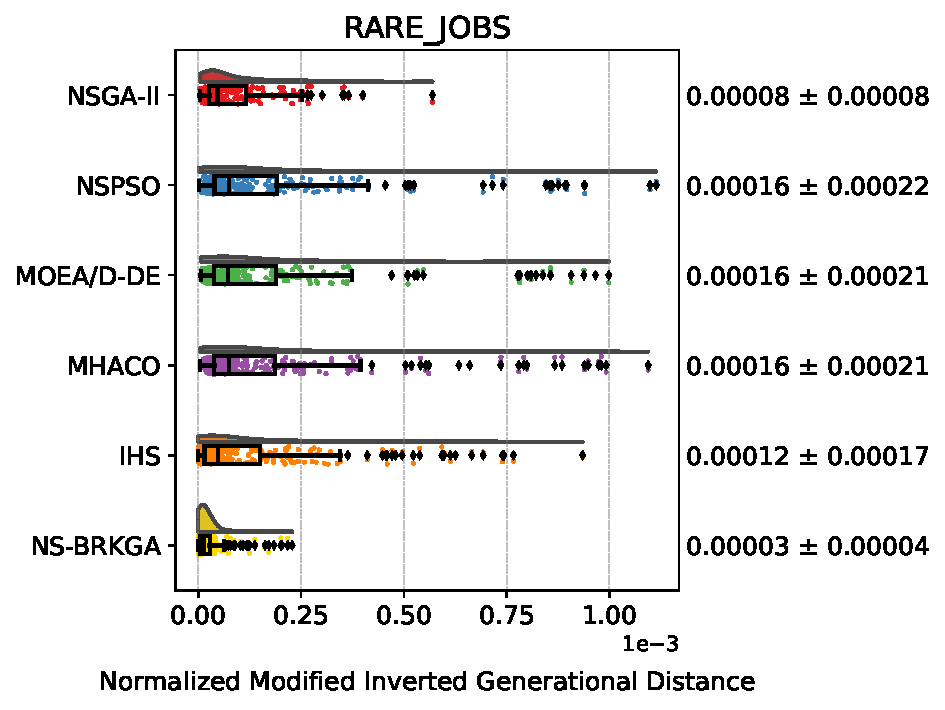
\includegraphics[width=0.88\textwidth]{figs/igd_plus_rare_jobs.pdf}
\end{figure}
\end{columns}

\takeaway{Em instâncias \texttt{rare}, NS-BRKGA é \textbf{3--6$\times$ melhor} em $\NIGDplus$ que os demais.}

\end{frame}

%========================================================================================
\section{Conclusão}

%----------------------------------------------------------------------------------------
\begin{frame}
\frametitle{Conclusões}

\begin{itemize}
\item Propusemos o \textbf{MOTMDSP}: extensão bi-objetivo do TMDSP para o trade-off entre makespan e tempo total de conclusão.

~\\

\item Desenvolvemos o \textbf{\textsc{NS-BRKGA}}: motor evolutivo independente do problema + decodificador guloso especializado.

~\\

\item Experimentos em \textbf{97 instâncias FOTA de larga escala}:\\
\textsc{NS-BRKGA} é consistentemente competitivo ou o melhor em $\HVR$ e $\NIGDplus$.

~\\

\item Especialmente forte em \textbf{instâncias \texttt{rare}}: maior robustez sob padrões irregulares de disponibilidade.

~\\

\item \textbf{Impacto prático:} fronteiras de Pareto diversas que ajudam tomadores de decisão a balancear throughput vs.\ tempo máximo.
\end{itemize}

\end{frame}

%========================================================================================
\begin{frame}[plain]
\begin{center}
{\Huge Obrigado!}

\bigskip\bigskip

{\LARGE Perguntas?}

\bigskip

\texttt{luis.mendes@ic.unicamp.br}
\end{center}
\end{frame}

%========================================================================================
\end{document}